% Original book diagram: fig:bayesian_inference
% Book source: sections/Part_I/bayesian_inference.tex
% Original diagram authorship retained. Visual design: Ziad Mosalam.
\documentclass[11pt,border=8pt]{standalone}
\usepackage{amsmath,amssymb,graphicx,tikz}
\usetikzlibrary{arrows.meta,automata,positioning,calc,shapes.geometric,fit,backgrounds,patterns}
\newcommand{\vect}[1]{\mathbf{#1}}
\newcommand{\mat}[1]{\mathbf{#1}}
\newcommand{\Normal}{\mathcal{N}}
\newcommand{\prob}{p}
\newcommand{\E}{\mathbb{E}}
\newcommand{\Var}{\mathrm{Var}}
\newcommand{\Cov}{\mathrm{Cov}}
\newcommand{\CovP}{\mathbf{P}}
\newcommand{\Prob}{\mathbb{P}}
\setlength{\textwidth}{6.5in}
% Shared visual vocabulary for the book's original diagrams.
% Figures opt in explicitly, so unrelated text and existing additions are unchanged.
\definecolor{BookBlue}{HTML}{003262}
\definecolor{BookGold}{HTML}{B17A00}
\definecolor{BookTeal}{HTML}{247C86}
\definecolor{BookInk}{HTML}{30363B}
\definecolor{BookLight}{HTML}{E9EFF5}
\tikzset{
  book figure/.style={font=\small\rmfamily, color=BookBlue, text=BookInk,
    line width=0.8pt, >=Latex},
  book axis/.style={->, draw=BookInk, line width=0.6pt},
  book link/.style={->, draw=BookBlue, line width=0.8pt},
  book observation/.style={draw=BookGold, fill=BookGold!8},
  book state/.style={draw=BookBlue, fill=BookLight},
  book note/.style={font=\footnotesize\rmfamily, text=BookInk}
}

\begin{document}
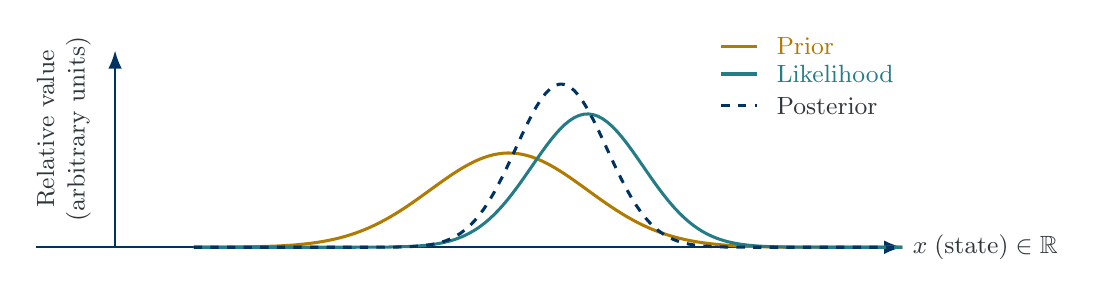
\begin{tikzpicture}[font=\small, text=BookInk, draw=BookBlue, line width=0.8pt, >=Latex, scale=1.0]
        \draw[->] (-1,0) -- (10,0) node[right] {$x \; (\text{state})\in \mathbb{R}$};
        \draw[->] (0,0) -- (0,2.5);
        \node[rotate=90, align=center] at (-0.65,1.5) {Relative value\\(arbitrary units)};

        % Curves drawn to scale for the example below (all densities scaled by 3).
% Prior N(5,1)
\draw[BookGold, line width=1.1pt, domain=1:10, samples=150]
plot (\x, {1.197 * exp(-(\x-5)^2/2)});

% Likelihood p(z=6 | x) with measurement variance 0.5
\draw[BookTeal, line width=1.1pt, domain=1:10, samples=150]
plot (\x, {1.693 * exp(-(\x-6)^2/1)});

% Posterior N(17/3, 1/3)
\draw[BookBlue, line width=1.1pt, dashed, domain=1:10, samples=150]
plot (\x, {2.073 * exp(-(\x-5.6667)^2/0.6667)});

        % Legend
        \begin{scope}[shift={(7.55,1.55)}]
            \filldraw[fill=white, draw=none] (0,0) rectangle (2.75,1.2);
            \draw[BookGold, line width=1.1pt] (0.15,1.0) -- (0.60,1.0);
            \node[text=BookGold, anchor=west] at (0.72,1.0) {Prior};

            \draw[BookTeal, line width=1.1pt] (0.15,0.65) -- (0.60,0.65);
            \node[text=BookTeal, anchor=west] at (0.72,0.65) {Likelihood};

            \draw[BookBlue, line width=1.1pt, dashed] (0.15,0.25) -- (0.60,0.25);
            \node[anchor=west] at (0.72,0.25) {Posterior};
        \end{scope}
    \end{tikzpicture}
\end{document}
